\documentclass{article}
\usepackage[utf8]{inputenc}
\usepackage{graphicx} % Required for inserting images
\usepackage{hyperref}
\usepackage{subcaption}
\usepackage{float}
\usepackage{tcolorbox}
\usepackage{amsmath}
\usepackage{amssymb}
\usepackage{listings}% http://ctan.org/pkg/listings}
\usepackage{algorithm}
\usepackage{algorithmic}
\usepackage[toc,page]{appendix}
\usepackage[backend=biber]{biblatex}
\usepackage{multicol}
\usepackage{siunitx}
\usepackage{comment}
\usepackage{xcolor}
\usepackage{caption}
\usepackage{tikz}
\usetikzlibrary{shapes.geometric, arrows}

\tikzstyle{startstop} = [rectangle, rounded corners, 
minimum width=3cm, 
minimum height=1cm,
text centered, 
draw=black, 
fill=red!30]

\tikzstyle{io} = [trapezium, 
trapezium stretches=true, % A later addition
trapezium left angle=70, 
trapezium right angle=110, 
minimum width=3cm, 
minimum height=1cm, text centered, 
draw=black, fill=blue!30]

\tikzstyle{process} = [rectangle, 
minimum width=3cm, 
minimum height=1cm, 
text centered, 
text width=3cm, 
draw=black, 
fill=orange!30]

\tikzstyle{decision} = [diamond, 
minimum width=3cm, 
minimum height=1cm, 
text centered, 
draw=black, 
fill=green!30]
\tikzstyle{arrow} = [thick,->,>=stealth]

% To delete lstlisting caption "Listing x"
%\captionsetup[lstlisting]{labelformat=empty}

\lstdefinestyle{myStyle}{
    belowcaptionskip=1\baselineskip,
    breaklines=true,
    frame=none,
    numbers=none, 
    basicstyle=\footnotesize\ttfamily,
    keywordstyle=\bfseries\color{green!40!black},
    commentstyle=\itshape\color{purple!40!black},
    identifierstyle=\color{black},
    backgroundcolor=\color{white},
}

\lstdefinestyle{cypherStyle}{
    backgroundcolor=\color{white},   % choose the background color
    basicstyle=\footnotesize\ttfamily,        % the size of the fonts that are used for the code
    commentstyle=\itshape\color{purple!40!black},
    keywordstyle=\bfseries\color{green!40!black},
    breakatwhitespace=false,         % sets if automatic breaks should only happen at whitespace
    breaklines=true,                 % sets automatic line breaking
    captionpos=b,                    % sets the caption-position to bottom
    commentstyle=\color{gray},    % comment style
    deletekeywords={},            % if you want to delete keywords from the given language
    escapeinside={\%*}{*)},          % if you want to add LaTeX within your code
    extendedchars=true,              % lets you use non-ASCII characters; for 8-bits encodings only, does not work with UTF-8
    %firstnumber=1000,                % start line enumeration with line 1000
    frame=none,                    % adds a frame around the code
    keepspaces=true,                 % keeps spaces in text, useful for keeping indentation of code (possibly needs columns=flexible)
    language=SQL,                    % the language of the code
    morekeywords={*,IF, REQUIRE, FOR, IS, LOAD, CSV, WITH, HEADERS, MERGE, toFloat, toInteger, date},            % if you want to add more keywords to the set
    numbers=none,                    % where to put the line-numbers; possible values are (none, left, right)
    numbersep=5pt,                   % how far the line-numbers are from the code
    numberstyle=\tiny\color{mygray}, % the style that is used for the line-numbers
    rulecolor=\color{black},         % if not set, the frame-color may be changed on line-breaks within not-black text (e.g. comments (green here))
    showspaces=false,                % show spaces everywhere adding particular underscores; it overrides 'showstringspaces'
    showstringspaces=false,          % underline spaces within strings only
    showtabs=false,                  % show tabs within strings adding particular underscores
    stepnumber=1,                    % the step between two line-numbers. If it's 1, each line will be numbered
    stringstyle=\ttfamily,     % string literal style
    tabsize=2,                       % sets default tabsize to 2 spaces
}

%% Golang definition for listings
%% http://github.io/julienc91/lstlistings-golang
%%
\lstdefinelanguage{Golang}%
  {morekeywords=[1]{package,import,func,type,struct,return,defer,panic,%
     recover,select,var,const,iota,},%
   morekeywords=[2]{string,uint,uint8,uint16,uint32,uint64,int,int8,int16,%
     int32,int64,bool,float32,float64,complex64,complex128,byte,rune,uintptr,%
     error,interface},%
   morekeywords=[3]{map,slice,make,new,nil,len,cap,copy,close,true,false,%
     delete,append,real,imag,complex,chan,},%
   morekeywords=[4]{for,break,continue,range,go,goto,switch,case,fallthrough,if,%
     else,default,},%
   morekeywords=[5]{Println,Printf,Error,Print,},%
   sensitive=true,%
   morecomment=[l]{//},%
   morecomment=[s]{/*}{*/},%
   morestring=[b]',%
   morestring=[b]",%
   morestring=[s]{`}{`},%
}

\lstdefinestyle{golangStyle}{
    captionpos=b,              % sets the caption-position to bottom
    belowcaptionskip=1\baselineskip,
    breaklines=true,
    frame=none,
    numbers=none, 
    basicstyle=\footnotesize\ttfamily,
    keywordstyle=\bfseries\color{green!40!black},
    commentstyle=\itshape\color{purple!40!black},
    identifierstyle=\color{black},
    backgroundcolor=\color{white},
    language=Golang,
}


\title{TFM-FernandoMartín}
\author{Fernando Martín Canfrán}
\date{April 2024}

\begin{document}

\subsection{Property Graph Design}

The property graph data model consists of two sub property graphs: a stable and a volatile property graph. On the one hand, the stable is composed of the most static part of the data that a bank typically gathers such as information about its clients, cards, ATMs (Automated Teller Machines). 
On the other hand, the volatile property graph models the transaction operations, which defines the most frequent and reiterative kind of interaction between entities of the data model.\\
The main difference and the main reason for this separation is the semantics with which we intentionally define each of the subgraphs: the stable will be understood like a fixed static bank database, whereas the volatile will be understood as the data model to define the transactions, as continuous interactions between the entities of the model, which won't be permanently saved, but instead, only for a certain window of time under the mission of detecting anomalous bank operations. Note that we will only model the transaction interaction in the volatile subgraph, only letting them occur here.
This separation will allow us to have a really simple and light property graph schema single-centered on the transactions with the minimal needed information (mostly identifiers of the entities a transaction links) and another, the stable, acting as a traditional bank database schema, from which to obtain the information details of the entities.

\subsubsection{Stable property graph}

Initially, we based our design in the artificial aforementioned Wisabi Bank Dataset \ref{}. Subsequently, although it is obvious that an actual banking data model is way more complex than the proposed one, the data model was simplified to the essential entities, relations and properties needed for the considered fraud detection patterns.

\begin{comment}
\begin{figure}[H]
    \centering
    \includegraphics[scale = 0.48]{PG-Design/images/diag-PG-stable-1.png}
    \caption{Initial stable property graph model}
    \label{img:pg-stable}
\end{figure}
\end{comment}

\begin{figure}[H]
    \centering
    \hspace*{-2cm}
    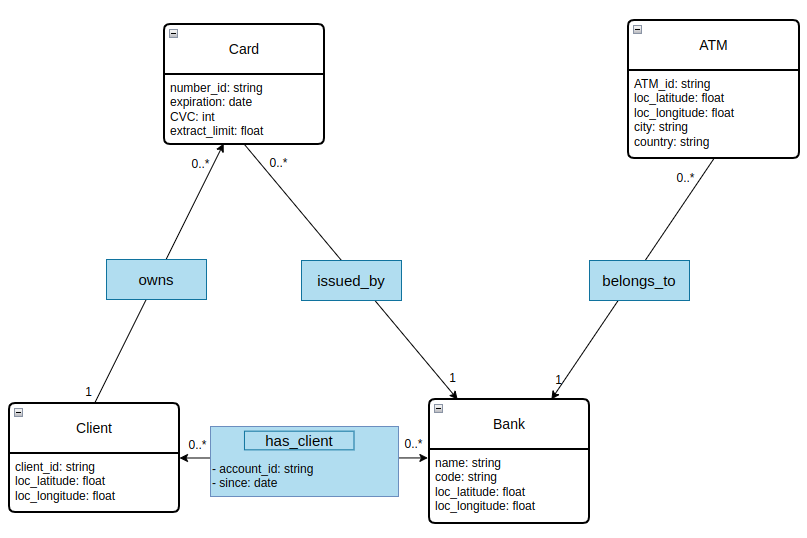
\includegraphics[scale = 0.45]{images/diag-PG-stable-updated.png}
    \caption{Initial stable property graph model}
    \label{img:pg-stable}
\end{figure}

% TODO: Cómo pongo que se entienda bien el 1er modelo y su correspondiente transformación al segundo y definitivo: explicando también en el medio las entidades, relaciones y atributos y su elección.
A first model proposal was the one shown in Figure \ref{img:pg-stable}. It contains four entities: Bank, ATM, Client and Cards, and the corresponding relations between them; in particular: a directed relationship from Client to Card: "owns" representing that a client can own multiple credit cards and that a card is owned by a unique client, then a bidirectional relation "has\_client" between Client and Bank; representing bank accounts of the clients in the banks. Then the relation between Card and Bank to represent that a Card is "issued by" a Bank, and that a Bank can have multiple Cards issued. Finally, the relation "belongs\_to" between the ATM and Bank entities, representing the ATMs that a Bank owns.

\begin{figure}[H]
    \centering
    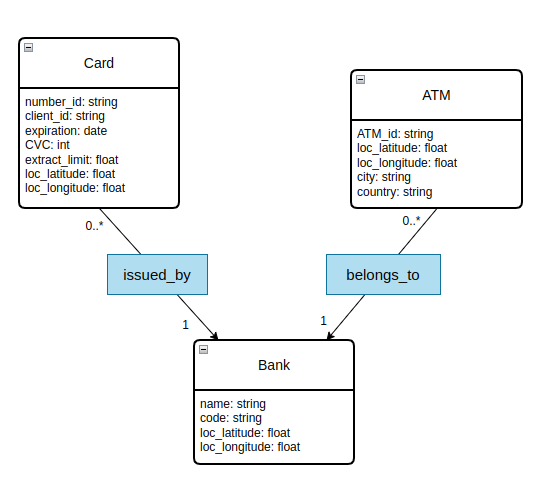
\includegraphics[scale = 0.6]{images/diag-PG-stable-def-updated.png}
    \caption{Definitive stable property graph model}
    \label{img:pg-stable-def}
\end{figure}

However, the final version of the model (see Figure \ref{img:pg-stable-def}) was simplified to reduce it to the minimal needed entities. In particular, Client entity was decided to be removed and included inside the Card entity. This reduction allows to simplify the stable property graph to only three entities. 
For this, all the Client attributes were included in the Card entity. In the initial Figure \ref{img:pg-stable} schema the Client entity was defined with three attributes: the identifier of the client and the GPS coordinates representing the usual residence of the client. This change is done while preserving the restriction of a Card belong to a unique client the same way it was previously done with the relation between Card and Client "owns" in the initial schema, which now is therefore removed. \\
% Account relation removed
Another derived consequence of this simplification is the removal of the other relation that the Client entity had with other entities: the "has\_client" relation between Client and Bank, which was originally made with the intention of representing the bank accounts between clients and banks. Maintaining a bank account would imply having to consistently update the bank account state after each transaction of a client, and, since for the so far considered fraud detection patterns we are not considering patterns related with the accounts, the removal of the bank account relation is negligible and at the same time helpful for the simplification of the model. However, for the sake of completeness the attribute \textit{extract\_limit} is introduced in the Card entity, representing a money amount limit a person can extract, which will be related with the amount of money a person owns. This will allow the detection of anomalies related with frequent or very high expenses.

The final entities and their selected attributes are described in what follows:

\paragraph{Entities\\}

\paragraph{Bank}

\begin{itemize}
\item[-] name: Bank name.
\item[-] code: Bank identifier code.
\item[-] loc\_latitude: Bank headquarters GPS-location latitude.
\item[-] loc\_longitude: Bank headquarters GPS-location longitude.
\end{itemize} 

\begin{figure}[H]
    \centering
    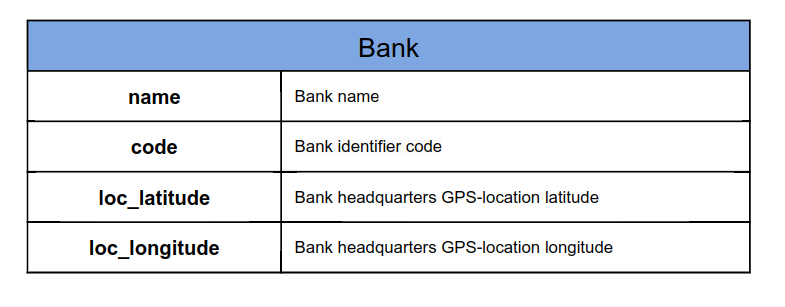
\includegraphics[scale = 0.4]{images/bank.png}
    \caption{Bank entity attributes}
    \label{img:pg-bank}
\end{figure}

\paragraph{ATM}

\begin{itemize}
\item[-] ATM\_id: Unique identifier of the ATM.
\item[-] loc\_latitude: GPS-location latitude where the ATM is located.
\item[-] loc\_longitude: GPS-location longitude where the ATM is located.
\item[-] city: City in which the ATM is located.
\item[-] country: Country in which the ATM is located.
\end{itemize}

\begin{figure}[H]
    \centering
    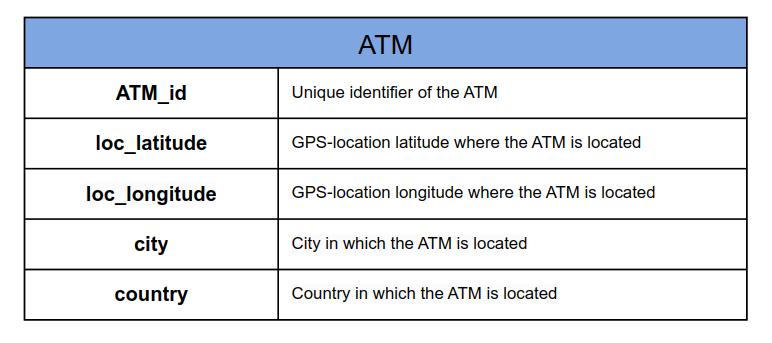
\includegraphics[scale = 0.4]{images/atm.png}
    \caption{ATM entity attributes}
    \label{img:pg-atm}
\end{figure}

% Potential possible generalization of the ATM entity to a POS entity
For the moment, this entity is understood as the classic Automated Teller Machine (ATM), however note that this entity could potentially be generalized to a Point Of Sale (POS), allowing a more general kind of transactions apart from the current Card-ATM transactions, where also online transactions could be included apart from the physical ones.

\paragraph{Card}

\begin{itemize}
\item[-] number\_id: Unique identifier of the card.
\item[-] client\_id: Unique identifier of the client.
\item[-] expiration: Validity expiration date of the card.
\item[-] CVC: Card Verification Code.
\item[-] extract\_limit: Limit amount of money extraction associated with the card.
\item[-] loc\_latitude: Client address GPS-location latitude.
\item[-] loc\_longitude: Client address GPS-location longitude.
\end{itemize}

\begin{figure}[H]
    \centering
    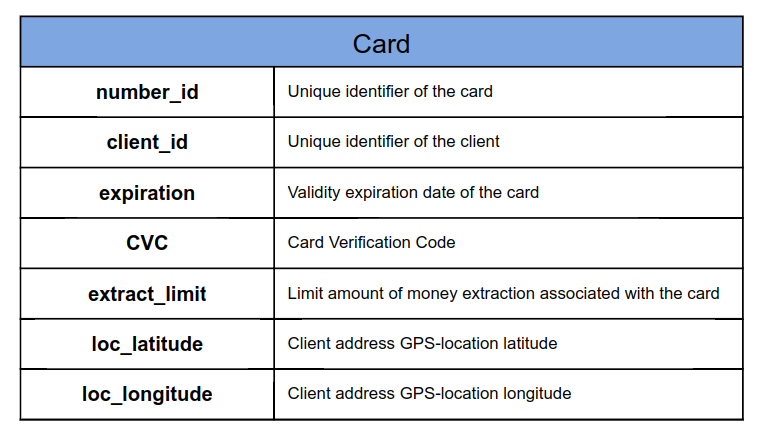
\includegraphics[scale = 0.4]{images/card.png}
    \caption{Card entity attributes}
    \label{img:pg-card}
\end{figure}

Note that for both the ATM and the Card entities we have the GPS coordinates information. In the first case referring to the geolocation of each specific ATM and in the last case referring to each specific client address geolocation. This will be useful to be able to detect transaction frauds related to geolocation distances.

Note that the client is completely anonymized in the system (no name, surname, age, or any other confidential details) by using only a client\_id. For the present purpose it is enough to uniquely identify each client.

% Relations -> and its attributes
\paragraph{Relations}
There are only two relations in the final stable subgraph, that is, the ones that are left after the deletion of the Client entity from the first version of the stable subgraph; the relation "issued\_by" between the Card and the Bank entities and the "belongs\_to" between ATM and Bank entities. For the moment they do not have any attribute, however they could potentially be added in the case this was needed.

\subsubsection{Volatile property graph}

It contains the minimal needed information to be able to recognize the anomaly fraud patterns we want to identify.
This subgraph describes the most volatile part of our model, meaning the transactions between the client's cards and the ATMs. The idea is to have a data model to define the transactions, as continuous temporal interactions between the Card and ATM entities, restricting these kind of relations to the volatile subgraph.
The idea is to have a really simple and light property graph schema single-centered on the transactions. For that the Card and ATM entities will be simplified to the last bullet, containing only the identifier of the both entities that each transaction relation matches. These identifiers will be enough to be able to recover, if needed, the whole information about the specific Card or ATM entity in the stable subgraph.

\begin{figure}[H]
    \centering
    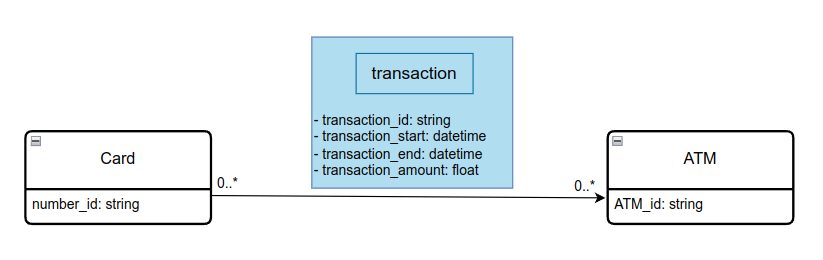
\includegraphics[scale = 0.45]{images/diagPG-volatile.png}
    \caption{Volatile property graph model}
    \label{img:pg-stable}
\end{figure}

Following this idea of volatile subgraph, the Card and ATM entities and transaction relations of it will not be permanently saved, but instead, only for a certain window of time under the mission of detecting anomalous bank operations. 

The transaction relation will include some attributes that will be essential for the detection of the fraud patterns, in particular:

\begin{itemize}
\item[-] transaction\_id: Unique identifier for each transaction in the database.
\item[-] transaction\_start: Datetime when the transaction started. Format: DD/MM/YYYY HH:MM (ex. 1/1/2022 4:50).
\item[-] transaction\_end: Datetime when the transaction was completed. Format: DD/MM/YYYY HH:MM (ex. 1/1/2022 4:54).
\item[-] transaction\_amount: Amount of money involved in the transaction.
\end{itemize}

\begin{figure}[H]
    \centering
    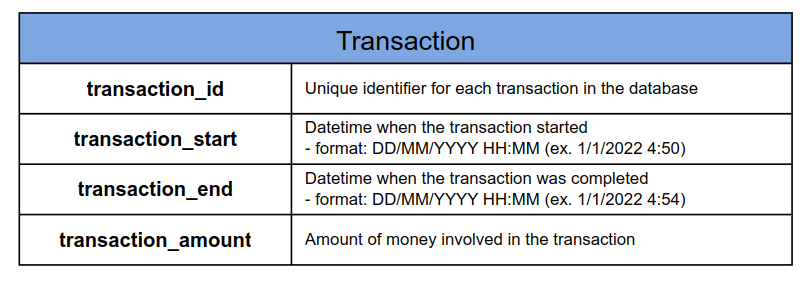
\includegraphics[scale = 0.40]{images/transaction.png}
    \caption{Transaction relation attributes}
    \label{img:pg-stable}
\end{figure}

\end{document}